\section{提案するサーバテスト手法}

構成管理ツール独立性とOS・ディストリビューション汎用性をいかに満たすかを考察する.

特定の構成管理ツールからの独立性を満たせない理由は2つある.ひとつは構成管理ツールがもつOS・ディストリビューション汎用性を利用するために,テストの実装が特定の構成管理ツールに依存していることである.

もうひとつはテストスイートでのテスト用VM構築フェーズが,特定の構成管理ツールのみ対応していることである.

OS・ディストリビューション汎用性が満たせないのは,テストがシェルコマンドを直接記述する実装になっており,OS・ディストリビューションの違いをテストコードを書く者自らが意識しないといけないからである.

この考察から,提案するテスト手法に必要な要件は以下の通りとなる.

\begin{enumerate}
  \item テストの実装を特定の構成管理ツールに依存しない
  \item テストスイートではなくテストのみに特化する
  \item OS・ディストリビューションの違いを利用者に意識させない
\end{enumerate}

そこでまずOS・ディストリビューション毎にコマンドを分離し,統一的なAPIでコマンドを呼び出すことができる汎用コマンド実行フレームワークを定義する.このフレームワークではまず構成管理ツール固有の振る舞い(パッケージインストール等)を抽出する.そして振る舞いをテストするためのAPIを定義する.更にAPIから呼び出されるコマンドをOS・ディストリビューション毎に定義する.APIとコマンド群の間にはOS・ディストリビューションを判別して自動で適したコマンドを返すレイヤーを設ける.


次に,テストコードの記述の抽象性を高め可読性を上げるために,宣言的な記法で汎用コマンド実行フレームワークを操作できる制御テストフレームワークを定義する.このフレームワークではまず記法の定義を行う.次に記法内の各命令と実際に呼び出す汎用コマンド実行フレームワークのAPIメソッドをひもづける.

汎用コマンド実行フレームワークと制御テストフレームワークの仕組みおよびその関係を\figref{fig:framework}に示す.

\begin{figure}[tb]
  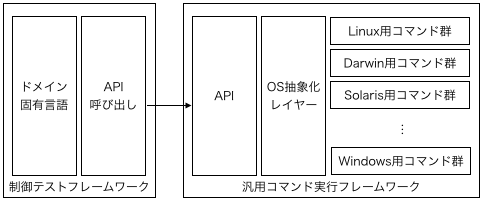
\includegraphics{framework-overview.png}
  \caption{汎用コマンド実行フレームワークと制御テストフレームワークの仕組みと関係}
  \label{fig:framework}
\end{figure}


この手法に基づき実装した汎用コマンド実行フレームワークをSpecInfra,制御テストフレームワークをserverspecと名付けた.

(ここからSpecInfraとserverspecの実装がどのようになってるのかを示す)
